%----------------------------------------------------------------------------------------
%
% LaTeX-template for degree projects at LNU, Department of Computer Science
% Last updated by Johan Hagelbäck, Mar 2017
% Linnaeus University
%
% License: Creative Commons BY
%
%----------------------------------------------------------------------------------------

%----------------------------------------------------------------------------------------
%	Settings and configuration
%----------------------------------------------------------------------------------------

\documentclass[a4paper,12pt]{article}

\usepackage[T1]{fontenc}
\usepackage{times}
\usepackage[english]{babel}
\usepackage[utf8]{inputenc}
\usepackage{dtklogos}
\usepackage{wallpaper}
\usepackage[absolute]{textpos}
\usepackage[top=2cm, bottom=2.5cm, left=3cm, right=3cm]{geometry}
\usepackage{appendix}
\usepackage[nottoc]{tocbibind}
\usepackage[colorlinks=true,
            linkcolor=black,
            urlcolor=blue,
            citecolor=black]{hyperref}

\setcounter{secnumdepth}{3}
\setcounter{tocdepth}{3}

\usepackage{sectsty}
\sectionfont{\fontsize{14}{15}\selectfont}
\subsectionfont{\fontsize{12}{15}\selectfont}
\subsubsectionfont{\fontsize{12}{15}\selectfont}
\usepackage{placeins}
\usepackage{csquotes} % Used to handle citations
\usepackage{pythonhighlight}

\renewcommand{\thetable}{\arabic{section}.\arabic{table}}  
\renewcommand{\thefigure}{\arabic{section}.\arabic{figure}} 

%----------------------------------------------------------------------------------------
%	
%----------------------------------------------------------------------------------------
\newsavebox{\mybox}
\newlength{\mydepth}
\newlength{\myheight}

\newenvironment{sidebar}%
{\begin{lrbox}{\mybox}\begin{minipage}{\textwidth}}%
{\end{minipage}\end{lrbox}%
 \settodepth{\mydepth}{\usebox{\mybox}}%
 \settoheight{\myheight}{\usebox{\mybox}}%
 \addtolength{\myheight}{\mydepth}%
 \noindent\makebox[0pt]{\hspace{-20pt}\rule[-\mydepth]{1pt}{\myheight}}%
 \usebox{\mybox}}

%----------------------------------------------------------------------------------------
%	Title section
%----------------------------------------------------------------------------------------
\newcommand\BackgroundPic{
    \put(-2,-3){
    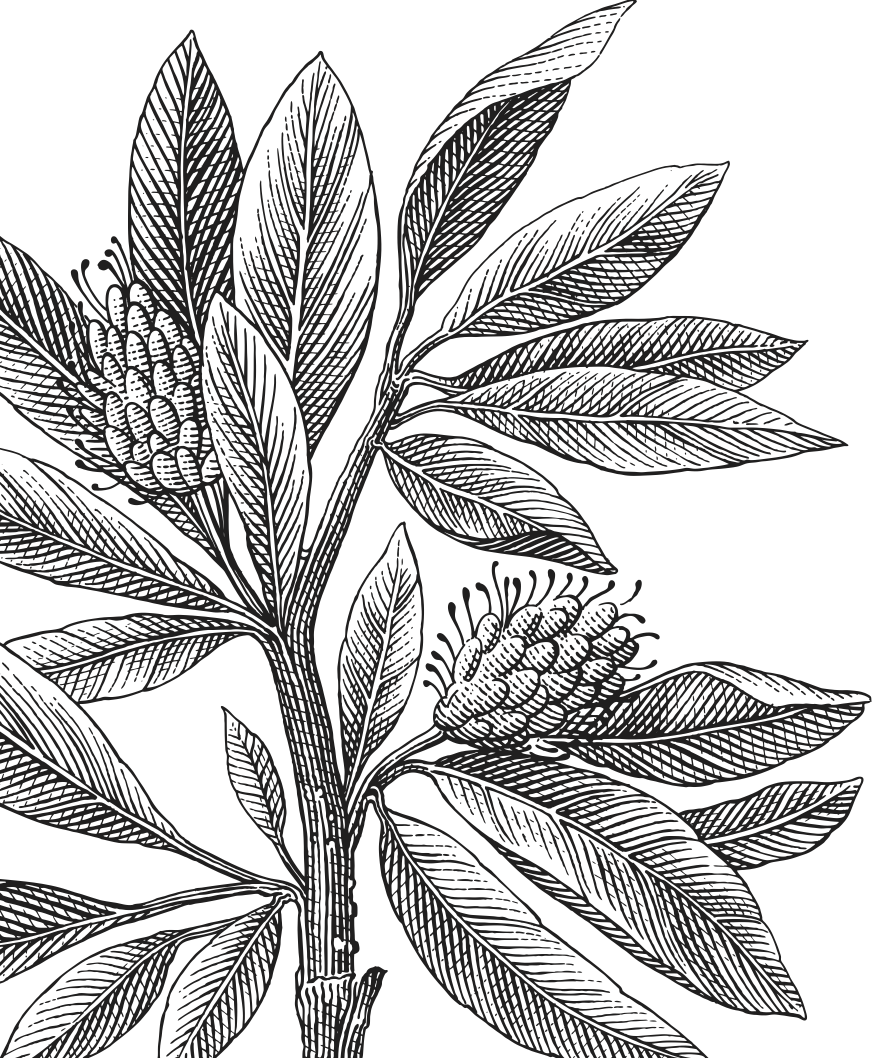
\includegraphics[keepaspectratio,scale=0.3]{img/lnu_etch.png} % Background picture
    }
}
\newcommand\BackgroundPicLogo{
    \put(30,740){
    
\includegraphics[keepaspectratio,scale=0.10]{img/logo.png} % Logo in upper left corner
    }
}

\title{	
\vspace{-8cm}
\begin{sidebar}
    \vspace{10cm}
    \normalfont \normalsize
    \Huge Bachelor Degree Project \\
    \vspace{-1.3cm}
\end{sidebar}
\vspace{3cm}
\begin{flushleft}
    \huge Evaluation of improvement measures of DNS Privacy\\ 
    \it \LARGE - Protection towards Web filters 
\end{flushleft}
\null
\vfill
\begin{textblock}{6}(10,13)
\begin{flushright}
\begin{minipage}{\textwidth}
\begin{flushleft} \large
\emph{Author:} Songho Lee\\ % Author
\emph{Supervisor:} Ola Flygt\\ % Supervisor
%\emph{Examiner:} Dr.~Mark \textsc{Brown}\\ % Examiner (course manager)
\emph{Semester:} VT 2019\\ % 
\emph{Subject:} Computer Science\\ % Subject area
\end{flushleft}
\end{minipage}
\end{flushright}
\end{textblock}
}

\date{} 

\begin{document}
\pagenumbering{gobble}
\newgeometry{left=5cm}
\AddToShipoutPicture*{\BackgroundPic}
\AddToShipoutPicture*{\BackgroundPicLogo}
\maketitle
\restoregeometry
\clearpage
%----------------------------------------------------------------------------------------
%	Abstract
%----------------------------------------------------------------------------------------
\selectlanguage{english}
\begin{abstract}
\noindent Current usage of the DNS system is the most significant loophole of Internet users' privacy, as all queries and answers for resolving web address are not protected in most cases. % Thesis statement, background description
Lack of confidentiality in the DNS system enables everyone who has control of the path between a user and DNS resolver can collect someone's usage pattern and fingerprint him and filter his access to specific websites. % Motivation
Despite a single solution for addressing privacy risks in all stages of the DNS query process does not exist, the report acquaints several Internet standardisations for DNS privacy that are complementary to the existing DNS system and verifies that implementation of these brings significant enhancement of users' privacy.
%The report explores existing methods to enhance DNS Privacy and sets up a series of experiments to verify implementations of such methods for privacy enhancement. % Description of problem explored
\\\\
\textbf{Keywords: DNS, DNS-over-https, DNS-over-TLS, Privacy}
\end{abstract}

%----------------------------------------------------------------------------------------
%	Preface
%----------------------------------------------------------------------------------------
%\newpage
%\textbf {\large{Preface}}\\

%\noindent You can have a preface in the report if you want, but it is not necessary. In this you can write more personal reflections on your degree project. In the preface you can also take the opportunity to thank the people who have been particularly helpful during the report writing, for example if you had any contact with a company that helped with the project, people that guided or helped you during the project, or your family and friends that supported you during the project. The preface shall not be longer than half a page.

%----------------------------------------------------------------------------------------
\newpage
\pagenumbering{gobble}
\tableofcontents % Table of contents
\newpage
\pagenumbering{arabic}

%----------------------------------------------------------------------------------------
%
%	Here follows the actual text contents of the report.
%
%----------------------------------------------------------------------------------------

\section{Introduction}
This chapter describes what Doname Name System (DNS) is, and how the legacy design of DNS has become a privacy threat. Before diving into the privacy risks of DNS, the background section introduces relevant structure and mechanisms. Knowledgable readers in DNS and Client subnet function may leap to section \ref{problemformulation}.

\subsection{Background}
Digital transformation has brought things used to be done in real life decades ago to the online. At work, people have a video conference call instead of a business trip if not necessary. For shopping goods, people fill in credit card numbers for cross-border payments rather than visiting a bank branch to issue paychecks. In other words, the stage where people work now has been shifted to cyberspace in recent decades, and the Internet has become an essential part of the people.

Despite the ubiquitousness of the Internet, users' activities online are collected under pervasive monitoring by different actors.
Pervasive Monitoring means ``widespread attack on privacy\cite{rfc7258}.'' Information collected in such action could lead to a breach of users’ privacy, by re-identifying users based on traffic\cite{herrmann2010analyzing}, or could become aids for launching an active form of attacks, such as masquerade and Denial of Service (DoS).
Unfortunately, insecure architecture of Domain Name System allows the pervasive monitoring, and thus it should be mitigated. Before discussing the privacy problems of DNS, we introduce DNS and its components which are important to adress.

\subsubsection{DNS}\label{dns-introduction}
Every activity on the web most likely begins with entering a human-friendly domain name in the web-browser. Once we enter a domain name for visiting a website, DNS resolves the address to an actual Internet Protocol Address of a web server which hosts the website. In case multiple websites are hosted on a single server, the entered fully qualified domain name(FQDN) is used to differentiate virtual hosts on a web server \cite{virtual24host}. Therefore, DNS is a critical component of the Internet.
%What about describing hjierarchical structure of Domain Name System here?
\subsubsection{DNS Servers}\label{dnsservers}
DNS servers consist of four types: Stub resolver, Recursive resolver, Authoritative server, and Forwarding DNS server. Resolvers refer to programmes that obtain information from name servers upon clients' requests \cite{rfc1034}.

Stub resolver is a resolver that serves as an entry-point of querying DNS from applications and directs search request to the nearest recursive resolver \cite{rfc1123}. As it cannot complete domain name resolution by itself, stub resolver is dependant on a recursive resolver \cite{rfc8499}.

The recursive resolver is a server which receives a DNS query from a stub resolver and gets the final answer to the query, by (1) answering from its local cache or (2) sending queries to other DNS servers \cite{rfc8499}. After a recursive resolver has sent a query request to other authoritative name servers, it is expected for the resolver to store the answer as a \textbf{local cache}. It is the first server in DNS query flow that contacts other servers to get the answer for the client. 

Authoritative (name) server is a server that has ``authority over one or more DNS zones \cite{rfc8499}'' and ``can answer queries without needing to query on other servers as it knows the content of the queried DNS zone by local knowledge \cite{rfc2182}.''

DNS forwarding server is a server that forwards queries to recursive resolver or other forwarding servers. It does not perform a query process for the stub resolver.
\subsubsection{DNS Query process}
Due to the hierarchical structure of the Domain Name System with delegations of authorities \cite{rfc1591}, getting the exact IP address of a given domain name involves several DNS servers. Figure \ref{queryprocess} shows an example of querying ``saimei.ftp.acc.umu.se.''. 
\begin{figure}[ht!]
    \begin{center}
        \includegraphics*[width=\columnwidth]{img/dnsquery}
    \end{center}
    \caption{DNS Query sequence diagram}
    \label{queryprocess}
\end{figure}
In the diagram, steps 2 and 3 returns top-level-domain(TLD) from the root servers. The steps 4 and 5 obtain the Authoritative name server of Swedish TLD. The .SE TLD returns name server of Ume\aa\ University in steps 6 and 7. In the last, the name server of umu returns IPv4 address (A record) of the given address, so that recursive resolver can provide the answer to the stub resolver. These steps are performed under the assumption that none of the queries is cached. 
\subsubsection{EDNS(0) and Client Subnet}
The extension mechanisms for DNS (EDNS) is specified in RFC 6891.
EDNS allows both DNS servers and client to send ``larger DNS packet than the original 512 octet limit \cite{rfc6891}'' so that it benefits of utilising larger size.
It makes sending long IPv6 address and possible DNSSEC signatures.
As of February 2019, major DNS resolver operators have started not to support non-EDNS compliant servers \cite{dns-flag-day, spacek-edns-camel-diet}. 

EDNS(0) provides several options, and one of the options is Client Subnet(ECS) feature, as described in RFC 7831 \cite{rfc7871}. When ECS is used, recursive DNS servers provide a truncated client IP address in its DNS queries to the upstream authorities to permit ``topologically localised answers for Content Delivery Networks (CDN) \cite{kintis2016understanding}''.
\subsubsection{CIA-triad}
In information security discussions, threat mitigations of a system are analysed in three perspectives: confidentiality, availability and integrity. These properties as a group are denoted as CIA triad or the security triad.
Achieving every aspect of CIA-triad often are not feasible, as enhancing one dimension may interfere with the other dimensions \cite{securityincomputing}.


\subsection{Related work}
The project accredits pioneer research of "DNS Privacy Considerations (RFC 7626) \cite{rfc7626}" which has provided theoretical foundations in analysis of DNS privacy. 
As of 2019, there are number of studies are presented to mitigate privacy issues based on the analysis. These studies are later presented in Chapter 3.

Survey of DNS privacy enhancing methods are presented by P. Werneck and J.H.C. van Heugten. P. Werneck evaluated approaches to improve privacy of DNS and stated limitations of identified approaches\cite{werneck2014dns} in 2014. J. Heugten evaluated exisiting solutions to ehnance DNS Privacy in 2018 in his study \cite{van2018privacy}. As standariseation of DNS-over-HTTPS is recently finalised\cite{rfc8484}, study from van Heugten reflects more recent changes.

\subsection{Problem formulation}\label{problemformulation}
Currently, almost all DNS traffic is sent in clear text \cite{rfc7626} over the UDP protocol \cite{tcp2014analysis}, and it makes DNS queries vulnerable to being hijacked or used to filter users' traffic.
All participants of the DNS query process, as illustrated in Figure \ref{queryprocess}, transmit messages intensively, and these are in plaintext.
It is also noteworthy that all participating authoritative name servers receive the same questions, although it is not necessary for Authoritative servers in higher hierarchies in the process to know all the complete domain address in question.

S. Bortzmeyer has analysed that particular fields in DNS packet\cite{rfc1035} such as Query name (QNAME) and Source IP address reveal ``communication relationships\cite{rfc7626}''.
These series of observations indicate that there are risks of information leakage in following places: (1) tapping on the wire ``between the stub resolvers and the recursive resolvers'', and (2) information leaks in the servers.
The following research questions are formulated having regards to the privacy breaching circumstances.

\begin{table}[h!]
    \begin{tabular} {|p{1.2cm}|p{12.8cm}|} \hline
        \textbf{RQ1} & Which are the use cases that the exisiting DNS Privacy enhancement methods could not address? \\ \hline
        \textbf{RQ2} & Which combination of different technologies would be suitable to address the limitation of the current status?\\ \hline
        \textbf{RQ3} & What would be possible disadvantages or overheads with DNS Privacy enrichment? \\ \hline
    \end{tabular}
    \caption{Research questions}
\label{researchquestions}
\end{table}

\subsection{Motivation}
Most of the internet activities begin with DNS query, hence DNS is vital. Notwithstanding the importance of DNS, designers of the current DNS protocol have not taken consideration of ``confidentiality of protocol metadata''. Therefore DNS queries reveal communication flows, and this property of DNS protocol is used in different contexts by different actors. Examples of usages are traffic monitoring for network management or limiting the influence of malicious websites by DNS Footprinting of malware\cite{stoner2010dns}, or detecting malware infections\cite{lemos2013got}.

Other exemplary usages of this property of DNS are nation-state surveillance, privacy-unfriendly activities of commercial sectors\cite{weaver2011redirecting}, and illegal actions by criminals. Surveillance affects individuals to possess stress and anxiety\cite{oulasvirta2012long}, and behavioural changes like self-censorship \cite{rfc6973}. RFC 6973 connotes that Privacy harms involve ``harms to financial standing, reputation, solitude, autonomy, and safety\cite{rfc6973}'' of individuals.

S. Farrell et al. state in RFC 7258 that allowing monitoring by benevolent actors and defending privacy against nefarious actors do not hold hand in hand, as the actions required to achieve both, regardless of the motivations, are indistinguishable\cite{rfc7258}.
Disadvantages incurred by lack of DNS privacy significantly overweight advantages, and therefore DNS privacy should be mitigated in any feasible practices.

\subsection{Objectives}
The following objectives are set to answer the research questions and transform the tasks into the smaller pieces. Hereafter we denote Objective as O and research questions as RQ, and Table \ref{objectives} shows the objectives which we will discuss.
\begin{table}[h!]
    \begin{tabular} {|p{1.2cm}|p{12.8cm}|} \hline
        \textbf{O1} & Explore the state of arts in mitigative methods to enhance DNS Privacy \\ \hline
        \textbf{O3} & Identify areas which the selected methods could not address. \\ \hline
        \textbf{O2} & Verify application of DNS privacy-enhancing methods complicates DNS eavesdropping\\ \hline
        \textbf{O4} & Estimate factors that may lead to a load increase on recursive DNS resolvers by improving DNS Privacy.\\ \hline
    \end{tabular}
    \caption{Objectives}
    \label{objectives}
\end{table}

RQ1 derives O1; mitigative methods need to be studied to see which methods exist.
O2 and O3 are set to answer RQ2; to see whether the methods we find by performing O1 helps to secure the privacy or not will prove any possible benefits of the Internet users. O4 aims to answer RQ3.
\subsection{Scope/Limitation}
The project has a focus on improving privacy part, from the security perspectives. In other words, reflected to a Confidentiality, Integrity, Availability(CIA) triad, enhancing Integrity and availability perspective is not priortised in the current project. Issues and challenges of DNS security as whole may be found in other studies, such as one conducted by Ning Hu et. al.\cite{ning2017dnssecurity}. 

%You cannot solve everything. Here you describe what you do, and what you don't do, in your project. Limitations can for example be that you only compare some frameworks of all frameworks available on the market, that you only suggest an architecture for a specific software product and not a general architecture, or that you only include university students in a study and not a broader population sample.

\subsection{Target group}
The project aims to provide insight on DNS Privacy for Internet users and recursive resolver providers for improving users' privacy.
%Here you outline which target group that might be interested in your work. If you, for example, do a project about software architectures, a target group can be professional developers and architects that work with similar software systems as the system you investigated.

\subsection{Outline}
The report follows in Introduction, Methods, Results, and Discussion(IMRaD) pattern. However, as several scientific methods are chosen, which is described in the next chapter, the result and analysis parts are extended for each chosen scientific method. 

\newpage
\section{Method}
\label{Method}
This chapter describes the chosen scientific methods to answer the research questions (see Table \ref{researchquestions}) and meet the objectives (see Table \ref{objectives}).
The study was conducted by systematic literature review and controlled experiment, and the following sections motivate the choice of a scientific method for meeting objectives. 
\subsection{Literature review}
A systematic literature review was performed to accomplish \textbf{O1} and \textbf{O3}; to study mitigative methods of DNS privacy and identify areas of limitations.
Exploring the existing design suggestions or implementation for improving the confidentiality of DNS transactions needed to be done systematically, to eradicate biases and to minimise opportunities for not obtaining suitable solutions.

A search criterium was set to list articles that cited RFC 7626 from a database Google Scholar, as the analysis had provided a clear insight of DNS privacy issues\cite{rfc7626}, and since around four years had passed after its publication, it was anticipated that fellow researchers have tried to solve or list risks identified in the article.
%If the results based on the criteria is insufficient, inclusive criteria will be applied using search term such as DNS Privacy and DNS Security will be used. Exclusive criteria must be applied as well to limit the contents of the articles to be relevant to the defined problem. Therefore, any solving other security aspects of DNS, such as availability or integrity will be excluded.
\subsection{Controlled Experiment and Verification}
\textbf{O2} was accomplished by selecting securing methods that are near or already in practice and reproduce these in a controlled environment.
Due to this reason, it may have excluded some of the areas from \textbf{O1}. Verification, as defined in \textbf{O2}, was done by Examining DNS query and response packets between stub resolver and recursive resolver, after having applied privacy enhancive methods under the controlled environment.

\textbf{O3} was achieved by studying surveys from \textbf{O1} and empirical results from \textbf{O2}. \textbf{O4} was evaluated based on outcome of \textbf{O1} and \textbf{O2}.

\subsection{Reliability and Validity}
The study is seen to have reliability on the results of the literature review, as the same effect will be derived by performing a search as described in the previous section. As Appendix A includes the source code of the experiment scripts, a similar result is expected to be derived by other researchers as well. 

The project deployed its experiments in a virtualised environment to minimise unforeseen factors that would impact performance measurements.

\subsection{Ethical considerations}
The project performed experiments in a controlled environment to eliminate other affecting factors. It means that no real data of legal representatives are collected without his/her consent. 

\newpage
\section{Survey of DNS Privacy enhancing methods}
This chapter presents the result of a systematic literature review on studies related to DNS Privacy.
%Afterwards, the analysis of the result follows.
As the raw data from the Google scholar had contained several duplicated entries, duplicated studies were excluded. Series or revisions of the same article are marked as duplicated. For such cases, the proceeding study was chosen to present.
The analysis section which follows after this chapter motivates strategies for categorisation of raw search results.

\subsection{Improvement suggestions}
Studies shown in Table \ref{channel} attempted to secure the communication channel of the DNS query. In other words, these studies suggested applying Encipherment mechanism to deliver Connection Confidentiality as X.800 defines \cite{x800}.

\begin{table}[h!]
    \begin{tabular}{ | l | p{10.5cm} | l | l | }
        \hline
            ID & Title & Year & Cites  \\ \hline
            \cite{hu2016specification} & Specification for dns over transport layer security (tls) & 2016 & 27 \\ \hline
            \cite{rfc8484} & Dns queries over https (doh) & 2018 & 5\\ \hline
            \cite{reddy2017dns} & Dns over datagram transport layer security (dtls) & 2017 & 3\\ \hline
            \cite{bucuti2015opportunistic} & An opportunistic encryption extension for the DNS protocol & 2015 & 2 \\ \hline
            \cite{dickinson2018usage} & Usage profiles for dns over tls and dns over dtls & 2018 & 1 \\ \hline
            \cite{saraj2017design} & Design and implementation of a lightweight privacy extension of DNSSEC protocol & 2017 & 0 \\ \hline
            \cite{dnsoquic} & Specification of DNS over Dedicated QUIC Connections & 2019 & 0 \\ \hline
            \cite{denis2015dnscrypt} & DNSCrypt & 2015 & 0 \\ \hline
            \cite{dempsky2010dnscurve} & DNSCurve & 2009 & 0 \\ \hline
        \end{tabular}
        \caption{Literatures categorised as securing communication channel}
\label{channel}
\end{table}

Table \ref{content} summarised studies on minimising privacy breaching information in the content of packets generated in the DNS query process.
%The approach can be seen as metaphors of Least common mechanism and Isolation as described in security design principles. 

\begin{table}[h!]
    \begin{tabular}{ | l | p{10.5cm} | l | l |}
        \hline
            ID & Title & Year & Cites \\ \hline
            \cite{bortzmeyer2016dns} & DNS query name minimisation to improve privacy & 2016 & 33 \\ \hline
            \cite{annee-dprive-oblivious-dns-00} & Oblivious DNS - Strong Privacy for DNS Queries & 2019 & 0 \\ \hline
            \cite{pan2018mitigating} & Mitigating Client Subnet Leakage in DNS Queries & 2018 & 0 \\ \hline
        \end{tabular}
        \caption{Literatures categorised as securing content}
\label{content}
\end{table}

There are several pieces of research and design proposals of new architecture which would replace the current DNS system. These are found in Table \ref{architectures}

\begin{table}[h!]
    \begin{tabular}{ | l | p{10.5cm} | l | l | }
        \hline
            ID & Title & Year & Cites \\ \hline
            \cite{ambrosin2018security} & Security and privacy analysis of national science foundation future internet architectures & 2018 & 3 \\ \hline
            \cite{grothoff2017gnunet} & The GNUnet System & 2017 & 1 \\ \hline
            \cite{asoni2017paged} & A Paged Domain Name System for Query Privacy & 2017 & 0 \\ \hline
            \cite{loibl2014namecoin} & Namecoin & 2014 & 12 \\ \hline
        \end{tabular}
        \caption{Literatures categorised as Architectural proposal}
    \label{architectures}
\end{table}
\FloatBarrier
\subsection{Case studies on attack scenarios}
Several studies demonstrated privacy risks of the current DNS standard and proposed mitigative methods which we had introduced in the previous section. 

\begin{table}[h!]
    \begin{tabular}{ | l | p{10.5cm} | l | l | }
        \hline
            ID & Title & Year & Cites \\ \hline
            \cite{kirchler2016tracked} & Tracked without a trace: linking sessions of users by unsupervised learning of patterns in their DNS traffic & 2016 & 10 \\ \hline
            \cite{mohaisen2017leakage} & Leakage of. onion at the DNS Root: Measurements, Causes, and Countermeasures & 2017 & 3 \\ \hline
            \cite{grothoff2017nsa} & NSA's MORECOWBELL: knell for DNS & 2017 & 3 \\ \hline
            \cite{spaulding2018d} & D-FENS: DNS filtering \& extraction network system for malicious domain names & 2018 & 1 \\ \hline
        \end{tabular}
        \caption{Literatures categorised as demonstrating attack scenarios by exploiting the lack of DNS privacy}
\label{attacks}
\end{table}
%\subsection{Evaluation of the improvement suggestions by other researchers}
\section{Analysis of DNS Privacy enhancing methods}
This section provides an analysis of the survey results.
The refined search results were categorised into the following fields: studies that suggested improving the security breach and investigations that demonstrated the security vulnerabilities.
We have further classified the privacy improving studies into ones securing the content and others enhancing the channel, based on the privacy risk analysis of RFC 7626.
S. Bortzmeyer, who is the author of RFC 7626, identified risk area of DNS privacy as the followings\cite{rfc7626}: 
\begin{enumerate}
    \item Data in the DNS request
    \item On the wire
    \item In the servers
    \item Re-identification and other Interferences
\end{enumerate}

\subsection{Securing the communication channel}
Communication channel encirpher methods, as we presented in Table \ref{content}, attempt to alleviate risks (2) on the wire. It also partially addresses risks of (4) re-identification depends on who the subject of the attacker is. 
However, we did not find the one simple solution for securing all communication paths of all involved parties of the DNS resolving. Therefore, the location of the DNS resolver needs to be considered when to mention the limitations of each suggested methods.

Let us abstract DNS query process into two phases, similar to van Heugten's approach \cite{van2018privacy}.
For ease of analysis, step 1 and 10 of Figure \ref{queryprocess} where stub resolver queries a domain name to the recursive resolver and the recursive resolver replies to the stub resolver (i.e. stub-to-resolver link) is defined as Phase 1.
Phase 2 denotes the rest of the steps which the recursive resolver resolves the queried address to concerning authoritative servers (i.e. recursive-to-auth link).

Common problems exist in channel encipher methods.
Most of the methods we found often do not encrypt communications on Phase 2 in contrast to Phase 1.
Furthermore, authentication mechanisms are missing on Phase 2 \cite{I-D.bortzmeyer-dprive-step-2}, and the lack of authentication of the authoritative server may potentially enable a Man-in-the-middle attack (MITM).

The fact that an authoritative server having a one-to-many server-client relationship from the recursive resolvers is the major obstacle of applying encryption on Phase 2.
As DoH \cite{rfc8484} and DoT \cite{hu2016specification} use Transport Layer Security (TLS) protocol \cite{rfc7858} for encryption, an authoritative server processing multiple TLS session is likely to end up exhausting its computational resources \cite{bhople2012server}, similar to a Distributed DoS (DDoS) attack situation. The issues are well discussed in the internet draft ``Next step for DPRIVE: resolver-to-auth link \cite{I-D.bortzmeyer-dprive-step-2}.''
% There are proposal of utilising TLS 1.3 and 

\subsubsection{Location of Recursive DNS resolvers}
From the end user's point of view, recursive DNS Resolvers can be on a local machine, one provided by the Internet Service Providers (ISP) and Public DNS servers \cite{van2018privacy}.
Selection of the location of recursive DNS resolvers leads to different impacts on the user's privacy, in terms of cache and obfuscation and logging. Section \ref{dnsservers} described caching on recursive resolvers.

\begin{figure}[ht!]
    \begin{center}
    \includegraphics*[width=0.6\columnwidth]{img/local-recursive}
    \end{center}
    \caption{A simplified network map when using local resursive resolver server.}
    \label{localrecursive}
\end{figure}
When a user utilises a local recursive resolver as illustrated in Figure \ref{localrecursive}, channel encipher methods do not add value to users' privacy considering that operations of phase two are often not encrypted.
Supposing that the user does not share local recursive resolver among the others, DNS queries which the user makes will not be fetched from a cache but all involved authoritative NS.
Sending queries in clear text on phase 2 leaves a possibility for all parties who are involved in the network packet transmission to monitor QNAME, query type and source IP of the traffic towards authoritative NS.
Referring to the assumption that local recursive resolver is unique for a person, there is no space for obfuscation since no one else is querying from the IP address of the recursive resolver.
However, utilising the local recursive resolver eliminates the risks of queries being logged (i.e. (3) risk in-the-servers) during Phase 1.


\begin{figure}[h!]
    \begin{center}
    \includegraphics*[width=0.6\columnwidth]{img/isp-recursive}
    \end{center}
    \caption{A simplified network map when using ISP-provided resursive resolver server.}
    \label{isprecursive}
\end{figure}
Using ISP provided Recursive resolver is the most common scenario, as most ISP offer DNS resolver to their users over Dynamic Host Configuration Protocol (DHCP).
The resolver from ISP is shared with other subscribers of the network, and it increases more chance of having queries cached by another user who acquired the address previously.
Reusing cache reduces the need of Phase 2 in its response process \cite{wang2013analysis} and thus generates less often-insecure traffics towards authoritative NS. 
Authoritative name servers see the source IP address of ISP's resolver in Phase 2 of DNS resolving, but not IP of the individuals, in case E-DNS Client Subset(ECS) is not in place.
When ECS is used, the authoritative NS may see truncated IP of clients\cite{kintis2016understanding}, but the IP address does not present additional privacy harm as ISP's recursive resolver is often in the same subnet IP range, and authoritative NS already acquaints source IP of the recursive DNS resolver. 
Privacy risks incurred by logging exist in ISP provided resolver, as ISPs may be obliged for log retentions due to legal requirements of the countries they operate in.

Channel encipherment on Phase 1 adds a value of users' privacy to a limited extent, tapping on the wire between the ISP's recursive resolver and a stub resolver is often feasible for ISP itself rather than third parties.

\begin{figure}[h!]
    \begin{center}
    \includegraphics*[width=0.6\columnwidth]{img/public-recursive}
    \end{center}
    \caption{A simplified network map when using public resursive resolver server.}
    \label{publicrecursive}
\end{figure}
Figure \ref{publicrecursive} briefly shows a scenario of using a public recursive resolver (as known as Public DNS resolver).
A public DNS server has more possibilities of being shared by a broader public compared to the ISP provided resolvers, and it increases the chances of queries being already cached. Authoritative servers see requests from the IP address of the public resolver, instead of stub resolvers' when ECS is not applied.

This scenario benefits users the most when channel encipherment is applied because DNS query contents in Phase 1 is not visible for parties in the middle of the networking path. It brings significant obfuscation in tracking down the end-user by analysing the network traffics. However, Public DNS servers may log the DNS queries and its client and therefore privacy risk that can occur (3) in-the-servers remains.

\FloatBarrier
\subsection{Securing content}
While applying the encipherment mechanism on the communications among DNS servers has a criticism that it only had only shifted the trust towards the Recursive resolver, applying design enhancements of packets' content brings significantly reduces the risks of (1) Data in the DNS request and data leaks in (3) the servers.
Query Name (QNAME) minimisation \cite{bortzmeyer2016dns} and Oblivious DNS \cite{annee-dprive-oblivious-dns-00} are the techniques of this category.

QNAME minimisation reduces the query leaks on higher authoritative name server chains, by presenting only relevant part of a domain name for an authoritative server to answer, instead of querying with FQDN.
It makes only relevant name server to acquire the full QNAME and query type. Therefore it reduces privacy risks on Phase 2.
Although the risk of data leaks still present in the last chain of the authoritative NS, this is less likely to happen unless a domain name owner has a malicious intent to exploit users' privacy.

\begin{figure}[h!]
    \begin{center}
    \includegraphics*[width=0.9\columnwidth]{img/ODNSoverview}
    \end{center}
    \caption{An overview of Oblivious DNS \cite{ODNSwebsite}}
    \label{odnsoverview}
\end{figure}
Oblivious DNS (ODNS) aims to decouple any association of a client IP address and DNS query content and no single party should be able to see both \cite{annee-dprive-oblivious-dns-00}. For this to work, it requires a special stub resolver and an ODNS authoritative resolver where the client creates a unique session key on each session to encrypt its DNS query and append 'odns' TLD. 

\newpage
\section{Privacy profiles}
Privacy is seen as having an access control in confidentiality in a security domain.
In everyday language, Privacy means ``the right to control who knows certain things about you \cite{securityincomputing}''.
Pfleeger introduces three aspects of Information security: sensitive data, affected parties, and controlled disclosure.
Privacy issues related to the DNS on different subjects are analysed in this chapter.

\subsection{Affected subjects}
The subjects are classified as private persons, and organisations. Organisations are further divided into large organisations that operate their directory server with DNS, and the smaller organisations that do not operate DNS resolvers in its network.

\subsection{Sensitive information}\label{sensitiveinformation}
Defining what sensitive information is in a subjective area.
Therefore, sensitiveness of the information cannot be measured on an absolute scale. However, several common areas of sensitive information follow.

For natural persons, EU has defined sensitive information as the following: personal data revealing ``(1) ethnic origin, religious or philosophical beliefs, (2) trade-union membership, (3) health-related data, and (4) data concerning a person's sex life \cite{GDPR}''.

For organisations, of their information, assets, especially copyright (expression of the idea), trade secret, and privileged information are examples of sensitive information \cite{securityincomputing}.

\subsection{Controlled disclosure}
The information has a different characteristic compared to any physical asset; it can be duplicated to an infinite amount at relatively low cost, without harming the asset.
This unique characteristic of information makes a ``propagation problem''.
Affected subjects lose control of the information about themselves after being disclosed.

\subsection{Privacy breaching Scenarios}
This section provides an analysis of the privacy breaching circumstances per affected subjects by observing DNS. Before focusing impacts on each subject, common privacy impacts are introduced by elaborating the privacy-related metadata.
Bortzmeyer highlighted that ``DNS data itself and a particular transaction'' should be confidential and transaction should not be public \cite{rfc7626}. The transaction refers to the DNS lookup in this context.
The following sections demonstrate how DNS reveals sensitive information about the affected subjects.

\begin{figure}[ht!]
    \begin{center}
        \includegraphics*[width=\columnwidth]{img/privacyobject}
    \end{center}
    \caption{Privacy related components on DNS transaction}
    \label{privacyobject}
\end{figure}

\subsubsection{Metadata in DNS query}\label{dnsmetadata}
Figure \ref{privacyobject} identifies relevant metadata created on DNS transaction.
The metadata created when looking up DNS record includes Query Name (QNAME or Request Name), Query type and client's IP address.
Contrary to the belief that metadata has only minimal information, the client IP address can be linked with WHOIS \cite{whois-icann}. Furthermore, geographical information of the client and affiliate of the organisation can be derived.

The recursive resolver can see whether the query is answered from its cache or not, and this information provides an insight into the client's behaviour.
Given a sufficient number of clients sharing the same recursive resolver, ``DNS queries on Chinese Top-Level-Domains(TLD) server had Zipf-like distribution \cite{wang2013analysis}''. If this phenomenon also applies to the rest of the TLDs, administrators of the recursive DNS resolver could infer that a user attempts to visit not-so-frequently-visited web server.

\subsubsection{Impact on individuals}
The Sensitive information related to the individuals can be derived by observing metadata created on DNS lookup process. The example scenarios are given in the order of information defined in section \ref{sensitiveinformation}.

There may be a domain shared mainly by people with shared philosophical beliefs if people are situated in countries with the legislation of censoring obligations on websites' administrators.
It is likely that people that share certain philosophical or political beliefs would host a dedicated website for holding a community rather than utilising censorship-enabled large social platforms \cite{mackinnon2009china}.
In such case, when a person visits such website, it may provide sufficient signal of the user's philosophical beliefs to those who can eavesdrop the traffic, although the detailed activities on such website are protected by encryption.

An employee visiting a certain trade-union's website frequently in a corporative network may indicate to an IT-department that either the person is a member of the union or has a sympathy with the organisation. 

Observing DNS query enables deriving health-condition of a user. If a chronic disease patient bears a smart sensor (such as Continuous Glucose Monitoring) that securely sends the measurement data to medical institutes \cite{carelink-uploading, medtronic-watson}, observing her DNS traffics may infer his health condition.
If someone actively visits several clinics that specialise in a particular disease and relevant medical insurance company's website, consequent DNS queries provide meaningful insight into the person's health status.

DNS queries related to online dating sites can also be observed. However, there has not found any evidence of potential sexual activity of individuals based on the frequency of the visit, without considering its sociosexuality \cite{sevi2018exploring}. 
Although the sexual activity cannot be derived, the sexual orientation of individuals could be induced in case the queried address is mainly visited among sexual minorities such as Grindr - the gay dating app \cite{goedel2015geosocial}.

\subsubsection{Impact on corporates/organisations}
The section illustrates privacy breaching scenarios for corporates' interest. First, scenarios of a large organisation are described. A common scenario regardless of the size of the organisations follows afterwards.

Assuming that large-scale enterprises have sophisticated intranet and employees are assigned with managed work laptops, an employee would utilise a web browser's bookmark to add company specific websites on his work computer.
In this case, although users do not necessarily visit the corporative intranet sites, a web browser may prefetch the bookmarks \cite{firefox-autocomplete-url, chrome-dns-prefectching}, which in its turn leaks the DNS queries.
If the employee was travelling, the leaked domain names have potentials to reveal employee's identity in public places by any observers, and the domain names can be collected to facilitate sophisticated and active attacks in the future.
In addition to the leaks caused by bookmarks from the browser, a query value `\textunderscore ldap.\textunderscore tcp.hostname' indicates that a client's dependency of a directory server \cite{Shulman:2014} and reveals the existence of service in the hostname.

Activities on new product development or sensitive assignment may be derived from the DNS query activities originated from the corporative IP address. Section \ref{dnsmetadata} mentioned about WHOIS record of IP addresses. Information on Autonomous System (AS) - administrative entity - might have a more substantial impact on identity linking on corporates compared to the individuals, once the information is correlated with the content of DNS Queries and frequency of the queries. Exchanging e-mails among various organisations or clients also involves DNS resolution and in this case Query type matters, since mail exchange server information is fetched by MX record of the DNS.

\subsection{DNS queries as a digital fingerprint}\label{fingerprint}
Kirchler et al. discuss possible ``behaviour-based-tracking'' of linking user sessions with the help of unsupervised learning of their DNS traffic patterns \cite{kirchler2016tracked}. Potential usage of such technique may especially be alarming for members of an organisation with critical missions, not only the private individuals.
Alongside with Kirchler's study, having an assumption that users would not change their recursive DNS resolver frequently, end-user reidentification based on web browsing history patterns \cite{olejnik2012johnny} could also be applicable in the context, as observing DNS query traffic provides a good representation of each client's web browsing history.
\newpage
\section{Design Constraints}
Applying channel encipherment methods for securing DNS queries such as using DNS-over-HTTPS or DNS-over-TLS implies that end-client gives trust in the chosen resolver. 
\newpage
\section{Design of controlled experiment}
This section describes the experimental setups, which consists of a choice of privacy enhancement methods to verify, and the way we verified these.

The survey presented in the previous section resulted in fruitful alternatives.
However, not all of them were in practical uses, with a reasonable amount of implementation on the server side.
As we analysed privacy impacts on the location of recursive resolvers, conducting experiments that cover several scenarios would be adequate. Thus, it is crucial to choose the solutions which both server and client implementation are available to test.
We reduced the scope of technologies to test to the followings implementations: DNS-over-HTTPS\cite{rfc8484}, DNS-over-TLS\cite{hu2016specification} and QName minimisation\cite{bortzmeyer2016dns}.

\subsection{Experiment scenarios}
Identifying incoming and outgoing traffics around a recursive resolver is our interest, as recursive DNS resolver knows about stub resolver's information and its query.
We previously analysed that the location choice of a recursive resolver leads to different value addition of privacy enhancement.
Scenarios where theoretically proven to have less value addition are not of our interest.
Therefore, in each experiment, we aim to verify situations where we anticipate privacy enhancement. 

\subsection{Verifying channel encipherment solutions}
We chose to use the remote recursive resolver (i.e. public DNS server) as the focus of the experiment laid on observing (2) on the wire traffic between the stub client and the resolver.

\subsubsection{DNS-over-HTTPS}
DoH clients that are available to test are Firefox web browsers later than version 62 \cite{FirefoxDoH}, curl later than 7.62 \cite{CurlDoH} and DNSCrypt-proxy. We apply each DoH client and generate DNS traffics as described in the Section \ref{simulation}. Afterwards, captured packets are analysed to see whether DNS queries of a client can be derived without putting efforts on intercepting encrypted traffics. Then captured packets are compared with the scenario where DoH client is not used.

\subsubsection{DNS-over-TLS}

\subsection{Verifying content enhancement solutions}
We deployed local recursive resolver since the focus of the test was to verify how securing contents of DNS queries contribute to enhancing end users' privacy. That will say, the experiment focused on analysing outgoing traffics from the recursive resolver to other authoritative DNS nameservers. 

The recursive resolver was set with a software BIND 9.14.0, as it is the most commonly deployed software for DNS servers and its latest version supports QNAME minimisation by default\cite{bind9qname}.
For this experiments, a controlled case is running DNS queries towards a BIND server which is configured to disable QNAME minimisation feature using, and an experiment case is performing the same steps to the server with QNAME minimisation enabled.

\subsection{Simulation of address resolution}\label{simulation}
We fetched a URL list of frequently visited websites as described in Appendix \ref{processweblist}.
We attempted to generate web traffic using a web automation tool as described in Appendix \ref{visitwebsites}.
However, since additional software is envolved for a traffics simulation, there is a chance that an error in the automation tool may lead to misleading results.
Therefore, we created a set of bookmarks from the method Appendix \ref{processweblist}, and visited the websites manually as well.

\begin{lstlisting}
    # sudo systemd-resolve --flush-caches
    # sudo systemd-resolve --statistics
    $ wireshark -i enp4s0 -k & python3 visitwebsites.py
\end{lstlisting}

\subsection{Tool to analyse the traffics}
We used Network traffic analytic tool, Wireshark to filter traffics based on the Port, and we abstract contents of the application layer and Internet Protocol layer to link clients' identities and their DNS transactions.
\newpage

\section{Results}
This chapter shows the result of verifying DNS Privacy solutions.
\subsection{DNS-over-HTTPS}
Figure \ref{selenium-mode2packets} shows a result of packet captures filtered with DNS (port 53) of a Firefox (66.0.2) simulation with Selenium which network.trr.mode is set as 2 and executed top 10 websites of 'de' domain.

\begin{figure}[h!]
    \begin{center}
    \includegraphics*[width=0.9\columnwidth]{img/selenium-firefox-mode2/wireshark}
    \end{center}
    \caption{Packet captures of Firefox where trust recursive resolver mode is enabled in mode 2}
    \label{selenium-mode2packets}
\end{figure}

%In this chapter you show and describe your results. You shall only show the raw results without any analysis, and you shall not put any conclusions or opinions in the description of the results. Try to be as objective as possible. An example of results from an experiment comparing five sorting algorithms is shown in Table \ref{results} below.\\


\newpage

\section{Analysis}
Results from Figure \ref{selenium-mode2packets} illustrates that none of the DNS queries is encrypted by using DNS-over-HTTPS when traffics are simulated using Selenium. This is suspected that Selenium simulation does utilise Firefox configuration profile that is applied to utilise DoH.

	
	
\newpage
	
\section{Discussion}
The project intensively examines securing Domain Name queries as a method of enhancing end-users' privacy towards pervasive monitoring.

\subsection{Why is DNS pointed out as a privacy leaking component apart from others?}
A Question may arise why it mainly focuses on securing DNS although there exist other factors which disclose users' privacy.
To answer the question, let us have an example of a web filter, as it is a commonly found practical example of the large scale monitoring\cite{murdoch2008tools}.
%As web filters require monitoring of users' traffic to enforce its policy of restrictions, understanding the mechanisms of the web filter suits this context.

Web filter, also known as content-control software, is software that restricts access to a content that is delivered on the Web.
Wazen et. al categorise mechanisms of legacy web-filtering into five techniques: (a) Port-based, (b) DNS, (c) IP Address, (d) Certificate, (e) Payload-based (f) HTTP proxy filtering techniques\cite{shbair2015efficiently}.
Except for the technique based on DNS filtering, the rest methods are regarded as well-mitigated due to recent developments of the web environment. 

Among the various types of filtering techniques mentioned above, methods (a) and (c) are considered less efficient due to changes in the Internet ecosystem in recent decennial;
Internet firms such as Google, Facebook and Amazon show strong presence\cite{haucap2014google}, and the phenomenon may have reduced the diversity of traffic endpoint's IP addresses.
Moreover, it has become more common to have web services deployed in cloud environments\cite{clouds2018stat}, and IaaS providers extensively use ``Virtual Host\cite{virtual24host}'', which means various Web servers correspond to the same IP address.
It also eliminates the need for utilising different ports to co-host services. Thus, port usages are normalised.

Also, another notable change of the Internet is that adoption of HTTPS on the web has increased significantly\cite{felt2017measuring}.
The change has increased costs of performing technique (e) and brought challenges in payload-based traffic classification \cite{xue2013traffic}.
Also, it has made (f) less applicable, as a proxy does not directly process encrypted traffics\cite{shbair2015efficiently}.
Furthermore, the combination of wide deployment of HTTPS and Virtual Hosting has made technique (e) inefficient, because ``many companies share the same certificate across different services and domain names\cite{shbair2015efficiently}''.

However, the trend change of Internet has not brought additional challenges to Domain Name System (DNS) filtering. Therefore, the project studies to remedy the weakest point towards users' privacy, which in this case is DNS.

%\subsection{Ethical dilemma of privacy enhancement; Liberation of illegal crimes?}
\subsection{Should end-users' IP considered as a person identifying information?}
People against of using ECS often argue that ECS may reveal an IP address of the end-user behind the DNS query, and therefore has a chacne of revealing the person's privacy.
However, it is doubted whether IP address itself should be seen as person identifiable factor, if subscription information is not linked by Internet Access Provider(IAP).
\newpage
		
\section{Conclusion}
In this chapter you end your report with a conclusion of your findings. What have you shown in your project? Are your results relevant for science, industry or society? How general are your results (i.e. can they be applied to other areas/problems as well)? Also discuss if anything in your project could have been done differently to possibly get better results. 

This chapter is also written in present tense.

\subsection{Future work}
You cannot do everything within the limited scope of a degree project. Here you discuss what you would do if you had continued working on your project. Are there any open questions that you discovered during the project work that you didn't have time to investigate?

\newpage


%----------------------------------------------------------------------------------------
%	References. IEEE style is used.
%
%----------------------------------------------------------------------------------------
\newpage

\hypersetup{urlcolor=black}
\bibliographystyle{IEEEtran}
\bibliography{references}
\newpage
%----------------------------------------------------------------------------------------
%	Appendix
%-----------------------------------------------------------------------------------------
\pagenumbering{Alph}
\setcounter{page}{1} % Reset page numbering for Appendix
\appendix

\section{Appendix 1}\label{processweblist}
This section describes the list of websites we simulated. The website list is fetched from Alexa top one million global chart and further classified depends on Top-Level-Domains (TLDs).
Below is code for a script to convert the Alexa list into a dictionary format.
\inputpython{../Selenium/process_web_list.py}{1}{30}

\section{Appendix 2}\label{visitwebsites}
This section includes a Python script for visiting websites using Selenium.
Selenium is the web automation test tool\cite{holmes2006automating}, which is typically used to test web applications. However, in our experiments, we utilised Selenium to visit a list of websites for simulating DNS queries. As we intended to use Firefox for DoH simulation, Selenium was incorporated with Firefox Gecko driver to control the web browser. Additionally, a Python script to operate Selenium.

Python 3.5 and higher, Pip3 is required. It is anticipated that Python packages such as selenium and json are also installed on the system. A Gecko driver needs to be reachable in OS' PATH environment. This code assumes that Firefox browser is installd on the local PC.

\inputpython{../Selenium/visitwebsites.py}{1}{70}
\section{Appendix 3}
Below is code for util.py which is a common base script.
\inputpython{../Selenium/util.py}{1}{110}
\end{document}
